\documentclass{article}
\usepackage[utf8]{inputenc}
\usepackage{indentfirst}
\usepackage{titling}
\usepackage{geometry}
\usepackage{graphicx}
\graphicspath{ {./Images/} }
\usepackage[shortlabels]{enumitem}
\usepackage{fancyhdr}
\usepackage{ulem}
\usepackage[dvipsnames]{xcolor}
\usepackage{amssymb}

\def\ojoin{\setbox0=\hbox{$\bowtie$}%
  \rule[-.02ex]{.25em}{.4pt}\llap{\rule[\ht0]{.25em}{.4pt}}}
\def\leftouterjoin{\mathbin{\ojoin\mkern-5.8mu\bowtie}}
\def\rightouterjoin{\mathbin{\bowtie\mkern-5.8mu\ojoin}}
\def\fullouterjoin{\mathbin{\ojoin\mkern-5.8mu\bowtie\mkern-5.8mu\ojoin}}

\renewcommand\maketitlehooka{\null\mbox{}\vfill} %para centralizar verticalmente
\renewcommand\maketitlehookd{\vfill\null}
\pagestyle{fancy}
\fancyhf{}
\rfoot{\thepage}
\lfoot{ 
\includegraphics[scale=0.01]{UA.jpg} José Mendes 107188 LEI}
\geometry{
  a4paper,
  headheight=4cm,
  top=5.5cm,
  bottom=4.5cm,
  footskip=4cm
}


\title{Complementos de Bases de Dados}
\author{José Mendes 107188}
\date{2023}

\begin{document}


\begin{titlepage}
    \maketitle
    \begin{center}
        
\includegraphics[scale=0.4]{UA.png}
    \end{center}
    \thispagestyle{empty} %remove o count da pagina
\end{titlepage}

\pagebreak
%depois por um index aqui

\section{Evolução dos Sistemas de Base de Dados}

\begin{flushleft}
    \textbf{Sistemas de Dados -} Cada vez mais as aplicações de hoje em dia
    são Data-Intensive, em vez de Compute-Intensive. 

    Para Data-Intensive, o poder bruto da CPU deixa de ser um fator limitante
    quando comparado com a \textbf{quantidade}, \textbf{complexidade} e \textbf{velocidade de atualização} dos dados.

    \vspace{3mm}

    De forma a otimizar a sua performance, um sistema de dados tipicamente oferece as seguintes
    funcionalidades:
    \begin{enumerate}
      \item \textbf{Bases de Dados -} armazenam os dados para utilização futura;
      \item \textbf{Caches -} guardam os resultados de operações dispendiosas, de forma a tornar a leitura mais rápida;
      \item \textbf{Search Indexes -} permitem aos utilizadores procurarem por palavras-chave ou filtrar os dados;
      \item \textbf{Message Queues -} permitem a comunicação assíncrona entre processos;
      \item \textbf{Stream Processing -} permite o processamento de dados em tempo real;
      \item \textbf{Batch Processing -} permite o processamento de dados acumulados, periodicamente;
    \end{enumerate}

    \textcolor{Blue}{Exemplo:}
    Um exemplo de \textbf{stream processing} ocorre na banca. Sempre que é realizada uma transação, os dados da mesma são
  imediatamente processados de forma a que o saldo esteja sempre atualizado.


  O \textbf{batch processing} é visível na faturação dos serviços pós-pagos pelas operadoras de telecomunicações. No final de
  cada mês, é feita uma consulta às suas bases de dados de forma a identificar todos os consumos do cliente, que são
  somados e depois gerada a fatura.


  No \textbf{stream} os dados são processados antes de armazenados, enquanto que no \textbf{batch} são processados depois de
  armazenados.

  \vspace{3mm}

  Cada vez mais as aplicações requerem um \textbf{maior wide-range de requisitos}. Muitas das vezes,
  \uline{uma única ferramenta já não consegue satisfazer todas as necessidades de \textbf{data processing} e \textbf{storage}}.

  \vspace{2mm}

  Em vez disso, o \uline{trabalho é partido em tasks que possam ser realizadas de forma eficiente
  por uma única ferramenta}. As ferramentas individuais utilizadas são depois juntas utilizando
  código de aplicação.

  \vspace{2mm}

  \textcolor{Blue}{Exemplo:} Podemos ter uma aplicação que utiliza uma Catching Layer (\textbf{memcached}), um Full-Text Search (\textbf{Elasticsearch})
  e uma Base de Dados principal separada (\textbf{MySQL}).
\end{flushleft}

\begin{center}
  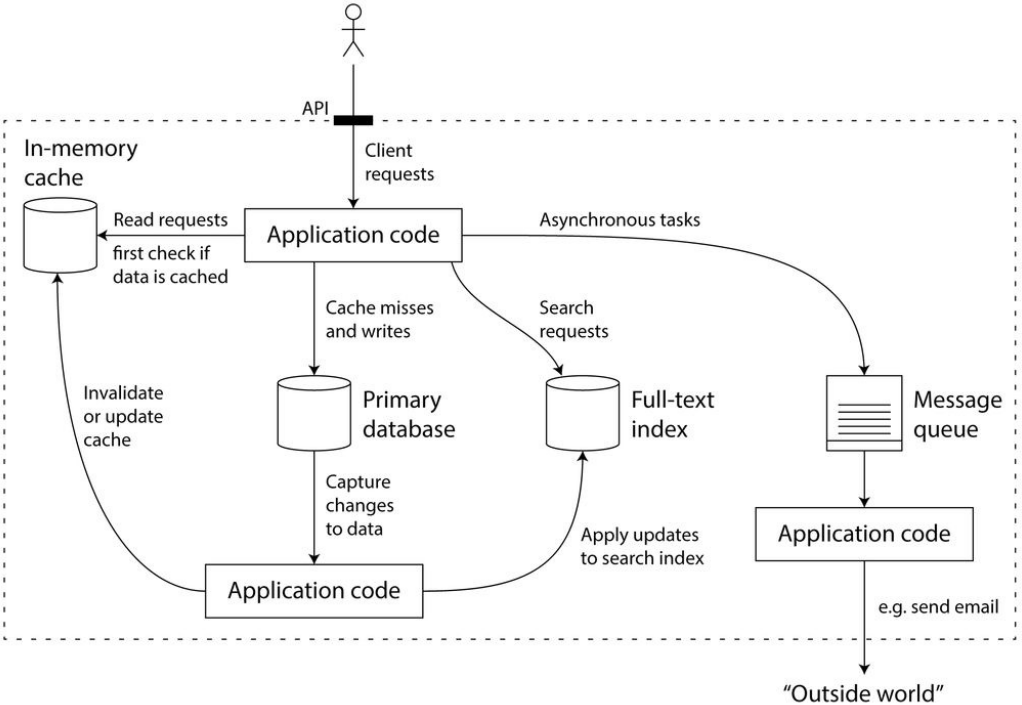
\includegraphics[scale=0.3]{1.png}
\end{center}

\subsection{Desafios que os Sistemas de Dados enfrentam}

\begin{flushleft}
  \item Como garantir que todos os dados se mantêm corretos e consistentes, mesmo quando, internamente, ocorreu algum erro? (ex: persistência de dados)
  \item Como fornecer boa performance para os clientes, mesmo quando partes do sistema estão degredadas?
  \item Como escalar o sistema para ser capaz de aguentar uma load intensiva de trabalho?
  \item Qual a aparência de uma boa API para o serviço?
\end{flushleft}

\subsection{Alguns Requisitos}

\begin{flushleft}
  \item \textbf{Fiabilidade -} O Sistema deve continuar a funcionar corretamente em caso de adversidades (ex: falhas de hardware, software ou mesmo humanas).
  \item \textbf{Escalabilidade -} O Sistema deve ser capaz de responder ao crescimento seja do volume de dados, do tráfego, ou mesmo da complexidade.
  \item \textbf{Manutenibilidade -} Deve ser possível que o Sistema sofra alterações ao longo do tempo por várias pessoas diferentes de forma produtiva.
\end{flushleft}

\pagebreak

\subsection{Bases de Dados}

\begin{flushleft}
  São definidas como um \uline{conjunto de dados relacionados entre si e a sua organização}.
  \vspace{2mm}
  Dividem-se em vários tipos, sendo atualmente os mais comuns: \textbf{Relacionais}, seguidas por
  \textbf{Documentais}, \textbf{Motores de busca}, \textbf{Chave-Valor}, entre outras. 
  \vspace{2mm}
  O controlo às bases de dados é realizado por \textbf{Sistemas de Gestão de Base de Dados} (\textbf{SGBD}
  ou DBMS em inglês). Estes fornecem funções que permitem a manipulação de grandes
  quantidades de informação.
\end{flushleft}

\section{NoSQL Databases - Key-Value Databases}

\begin{flushleft}
  \begin{enumerate}
    \item É o mais simples dos tipos NoSQL;
    \subitem Consiste apenas em chaves únicas e a um "bucket" que contêm qualquer tipo de dados que se pretenda;
    \item Pares chave-valor:
    \subitem \textbf{Chave}: (id, identificador, chave primária) Normalmente é uma String;
    \subitem \textbf{Valor}: Pode ser qualquer tipo de dados, texto, estrutura, imagem \dots;
    \item O conteúdo do valor ("bucket") pode ser, literalmente, qualquer coisa (mais comum é não estruturado ou semi-estruturado);
    \item Os "buckets" podem armazenar entradas pesadas, incluindo BLOBs (Basic Large Objects);
    \item Row based systems, utilizados para eficiência;
  \end{enumerate}
\end{flushleft}

\subsection{Vantagens}

\begin{enumerate}
  \item Tolerância a falhas elevada - sempre disponível;
  \item Schemaless, logo, muito flexível. oferece uma grande escalabilidade para mudar os requisitos dos dados;
  \item Eficiente a devolver dados de um objeto, com operações de disco minimas;
  \item Muito simples, rápido e fácil de dar deploy;
  \item Ótimo para escalabilidade horizontal (muitos servidores);
  \item Não necessita de queries SQL, indexes, triggers, sp's, views, \dots;
  \item Data ingest rates muito elevadas (muitos dados a entrar);
  \subitem Favorece: escreve uma vez, lê muitas vezes;
  \item Potente no "offline reporting" com data sets muito grandes;
  \item Existem formas avançadas de KVs que apresentam capacidades de document ou column oriented stores;
\end{enumerate}

\pagebreak

\subsection{Desvantagens}

\begin{enumerate}
  \item Não é apropriado para aplicação complexas;
  \item Não é eficiente a ataualizar records em que apenas parte do "bucket" é alterado;
  \item Não é eficiente em devolver informação limitada de records específicos (ex: returning only
  records of employees making between \$40K and \$60K); 
  \item Não é apropriado para queries complexas;
  \item Com o aumento do volume de dados, manter chaves únicas pode tornar-se um problema;
  \item Geralmente precisa de ler todos os records de um "bucket" ou talvez precise de contruir índices secundários;
\end{enumerate}

\subsection{Use Cases}

\begin{enumerate}
  \item Session data, user profiles, user preferences, shopping
  carts, \dots;
  \item Criar datasets que são raramente acessados mas crescem ao logo do tempo (Caching);
  \item Onde a performance de escrite é a prioridade;
\end{enumerate}

\subsection{Quando NÃO usar}

\begin{enumerate}
  \item Quando precisamos de ter relações entre entidades;
  \item Queries requerem acesso a conteúdos da parte dos valores;
  \item Set operations que envolvem múltiplos pares chave-valor;
\end{enumerate}

\subsection{Key Management}

\begin{flushleft}
  Como devem as chaves serem produzidas?

  \item \textbf{Manualy assigned keys} - Identificadores do mundo real (ex: e-mail, login names, \dots);
  \item  \textbf{Automatically generated keys} - Auto-incremente integers ou chaves mais complexas geradas por algotitmos;
\end{flushleft}


\pagebreak

\subsection{Query Patterns}

\begin{enumerate}
  \item Basic \textbf{CRUD} operations;
  \subitem Apenas quando a chave for dada;
  \subitem O conhecimento da chave é essencial;
  \subitem Ás vezes, pode ser até dificil para uma base de dados dar uma lista com todas as chaves;

  \item \textbf{No searching by value};
  \subitem Mas pode-se instruir à base de dados como dar parse aos valores, para fazer operações;

  \item \textbf{Batch / sequential processing}
  \subitem MapReduce;
\end{enumerate}

\subsection{Outras funcionalidades}

\begin{enumerate}
  \item Expiração de  pares chave-valor;
  \item Coleções de valores (We can store not only ordinary values, but also their
  collections such as ordered lists, unordered sets etc.);
  \item Links entre pares chave-valor (podem ser usados quando se usa queries);
\end{enumerate}

\subsection{Exemplos}

\begin{enumerate}
  \item \textbf{RiakKV}
  \item \textbf{Redis}
\end{enumerate}

(Ver slides 12-40)

\section{NoSQL Databases - Document Databases}

As bases de dados de documentos são bastante eficientes em cenários \textbf{one-to-many}.
Oferecem um esquema flexível (mesmo dentro das mesmas coleções (informação heterogénia)) e melhor performance
(devido ao armazenamento da informação junto à entidade a que esta se refere) que são
manipulados através de código simples.

\begin{flushleft}
  \textbf{Nota:} A flexibilidade permite que existam objetos na mesma coleção com atributos ligeiramente diferentes, sem necessidade
  de criarmos uma tabela para cada tipo de objeto.

  A localidade pode levar à duplicação de dados entre documentos.
\end{flushleft}

Um \textbf{documento} caracteriza-se por uma \textbf{string continua} codificada em JSON, XML,
ou outro formato binário estruturado.
É self-described (atributos são claros) e apresentam uma \textbf{estrutura em árvore}. São
identificados por um \textbf{id único}.

Geralmente, para manipular, é necessário carregá-lo por completo e para guardar as
alterações reescreve-lo na totalidade.

\begin{flushleft}
  \textbf{Nota:} A localidade só se torna uma vantagem se manipularmos porções grandes do documento.
\end{flushleft}

\pagebreak

Esta topologia não aplica a modelos \textbf{many-to-many}, pois não existem
operações de \textbf{join} de documentos. Deve também ser evitada quando a estrutura
do documento é demasiado instável (sempre a mudar).

\begin{flushleft}
  \textbf{Nota:} Não é desejável demasiada granularidade entre os documentos porque se todos apresentarem características
  diferentes não são relacionáveis e assim não fará sentido estarem na mesma coleção.
\end{flushleft}

No entanto, é a ideal para logging de eventos, sistemas de gestão de conteúdos,
blogues, web analytics, aplicações e-commerce \dots
Por ser a solução para alguns, mas não para todos os problemas, as bases de dados
relacionais começaram a incluir funcionalidades documentais e vice-versa.

\subsection{Exemplos}
  \begin{enumerate}
    \item \textbf{MongoDB}
    \item \textbf{CouchDB}
    \item \textbf{Couchbase}
  \end{enumerate}
  (Ver slides 11-51)

\section{Modelos de bases de dados}

Os modelos de dados com os quais os programas vão trabalhar têm um papel fundamental na
sua programação.
Têm um efeito enorme na forma como os programas são escritos e na forma como
nós pensamos sobre os problems que estamos a resolver. Todos os modelos de dados
têm formas diferentes de representar os dados e de os manipular.

\subsection{Bases de Dados Relacionais}

Este tipo de base de dados oferece vários benefícios (resolvendo a maior parte dos problemas com dados), entre os quais a \textbf{persistência} dos dados (ao guardar dados eles mantêm-se guardados),
a \textbf{integração} com várias aplicações (com a mesma DB) e a \textbf{atomicidade}, \textbf{consistência}, \textbf{isolamento} e \textbf{duranilidade}
oferecidas pelas \uline{transações} (ACID).

\subsubsection{Transactions - ACID Properties}

\begin{itemize}
  \item \textbf{Atomicidade} - Numa transação, ou todas as operações são executadas, ou nenhuma é;
  \item \textbf{Consistência} - É garantido que as restrições de integridade
  antes da transação se mantêm após esta;
  \item \textbf{Isolamento} - As alterações feitas na BD só são visíveis quando a transação termina.
  \item \textbf{Durabilidade} - Assim que commited, as alterações de uma transação persistem mesmo em caso de falhas.
  
  A durabilidade é garantida através das
transactions log, que permite a recunstrução das transações perdidas em caso
de falhas.
\end{itemize}

\pagebreak

\begin{center}
  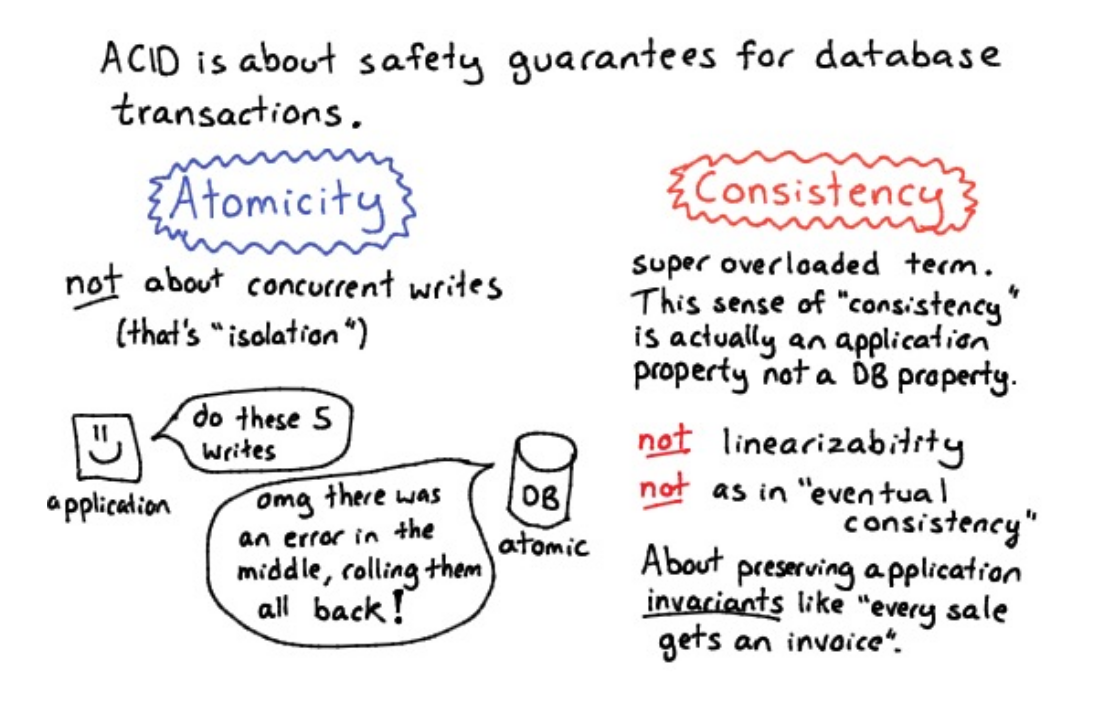
\includegraphics[scale=0.3]{2}
  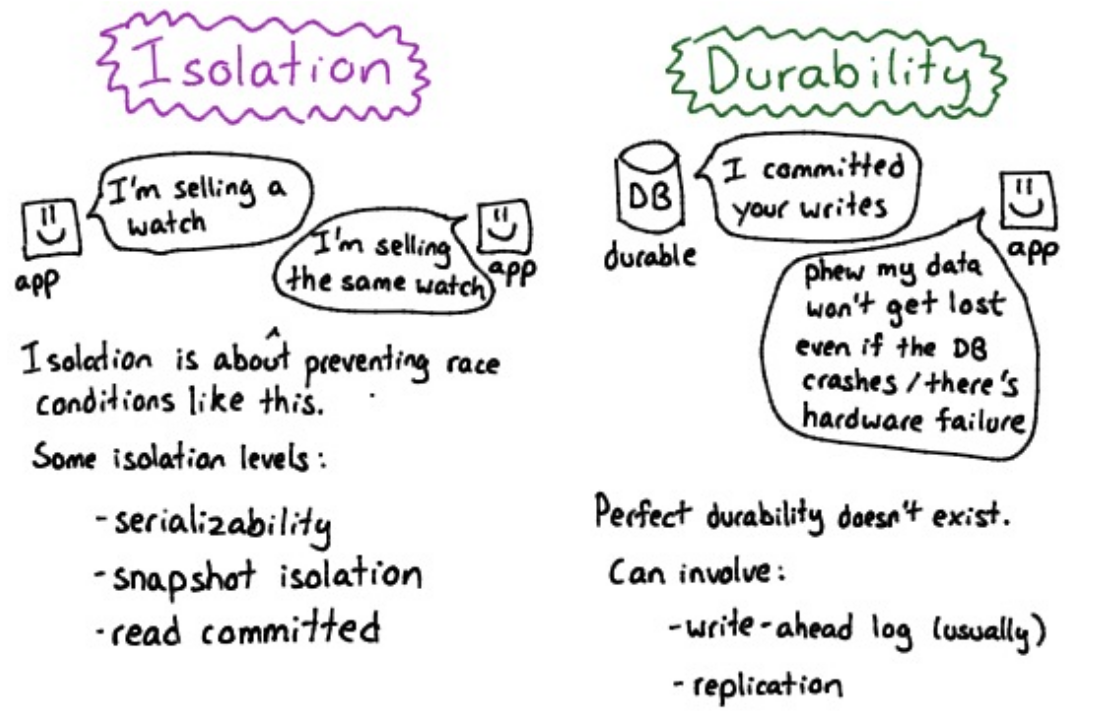
\includegraphics[scale=0.3]{3}
\end{center}

(Ver slides 7-8, história das bases de dados relacionais)

\pagebreak


\subsection{Current Trends and Issues}

\begin{flushleft}
  Algumas trends e issues motivaram à mudança nas tecnologias de armazenamento
de dados relacionais (em use cases e na tecnologia).

\textbf{Key Trends include:} Aumentar o volume de dados e tráfego. Ligação entre dados mais complexo.
\textbf{Key Issues include:} O problema $\rightarrow$ \textbf{impedance mismatch}.
\end{flushleft}

\subsection{Impedance Mismatch}

Nos últimos tempos, tem-se assistindo a um \textbf{aumento do volume de dados e tráfego}, a par da
redução do relacionamento entre eles, ou seja, \textbf{cada vez há mais dados não relacionados}.

Tem-se também verificado um conflito entre os \uline{princípios de engenharia de
software}, onde o
paradigma é \uline{orientado a objetos} e os princípios relacionais baseados em \uline{modelos
matemáticos}. Este problema é designado por \textbf{Impedance} (oposição que um circuito elétrico faz à passagem de corrente elétrica quando é submetido a tensão)
\textbf{Mismatch} (Disparidade, incompatibilidade).

Atualmente, este verifica-se nas estruturas isoladas, que violam os princípios da \textbf{normalização}.
Para armazenar informação persistentemente em programas modernos, uma única
estrutura lógica tem de ser separada (\textbf{normalização}).

\subsubsection{Exemplo}

Vários objetos que representem funcionários numa empresa. Cada funcionário terá o seu departamento,
mas vários funcionários podem trabalhar no mesmo departamento. Se a base de dados refletir o paradigma orientado a
objetos, iremos ter uma repetição dos departamentos nos vários funcionários e base de dados não estará normalizada!

No entanto, fazer múltiplos selects e joins para construir uma entidade às vezes não é a melhor opção.

\begin{center}
  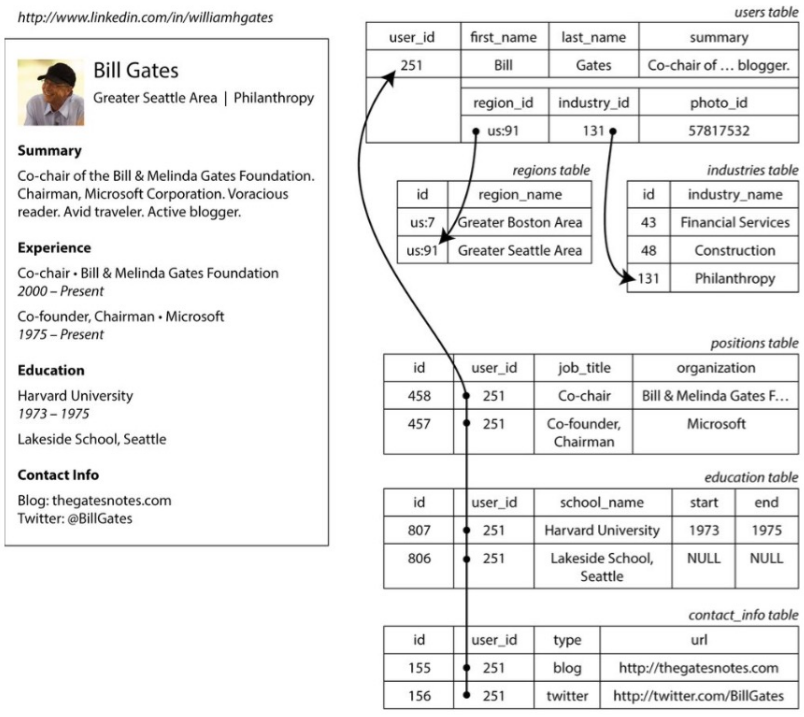
\includegraphics[scale=0.3]{4}
\end{center}

\pagebreak

\subsubsection{One-to-Many relations}

\begin{center}
  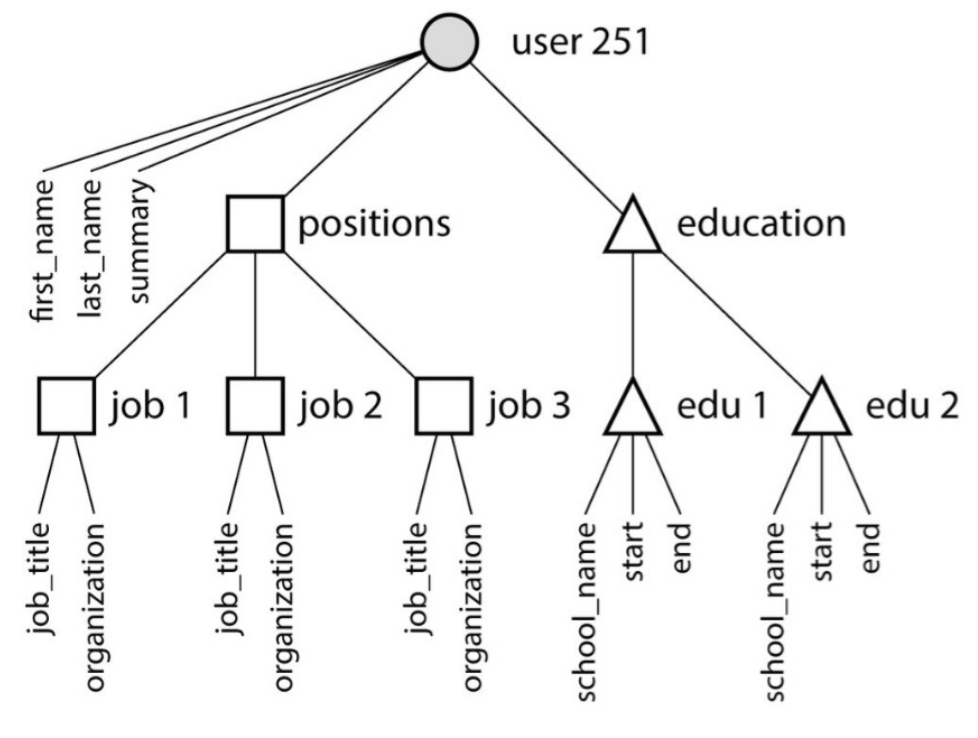
\includegraphics[scale=0.2]{5}
\end{center}

\subsection{Normalização}

Tem o objetivo de \textbf{reduzir a redundância dos dados}.
Em DB's este reflete-se na \uline{utilização de IDs} para identificar entidades,
oferecendo uma \textbf{consistência de utilização}, ao mesmo tempo que
\textbf{previne ambiguidades}, caso hajam entidades semelhantes (ex: com o mesmo nome),
\textbf{facilita alterações} das entidades, uma vez que a sua informação está armazenada
numa única tabela, motivo pelo qual também \textbf{facilita a tradução}.

\begin{flushleft}
  \textbf{Nota:} Uma base de dados que verifica estas características diz-se \textbf{normalizada}.
  Uma base de dados na qual as entidades como região e industria estão referidas
  por ID diz-se \textbf{normalizada}.

  No entanto, uma basde de dados que duplica nomes e propriedades de entidades
  em cada documento diz-se \textbf{desnormalizada}.
\end{flushleft}

\subsubsection{Many-to-Many relationships}

\begin{center}
  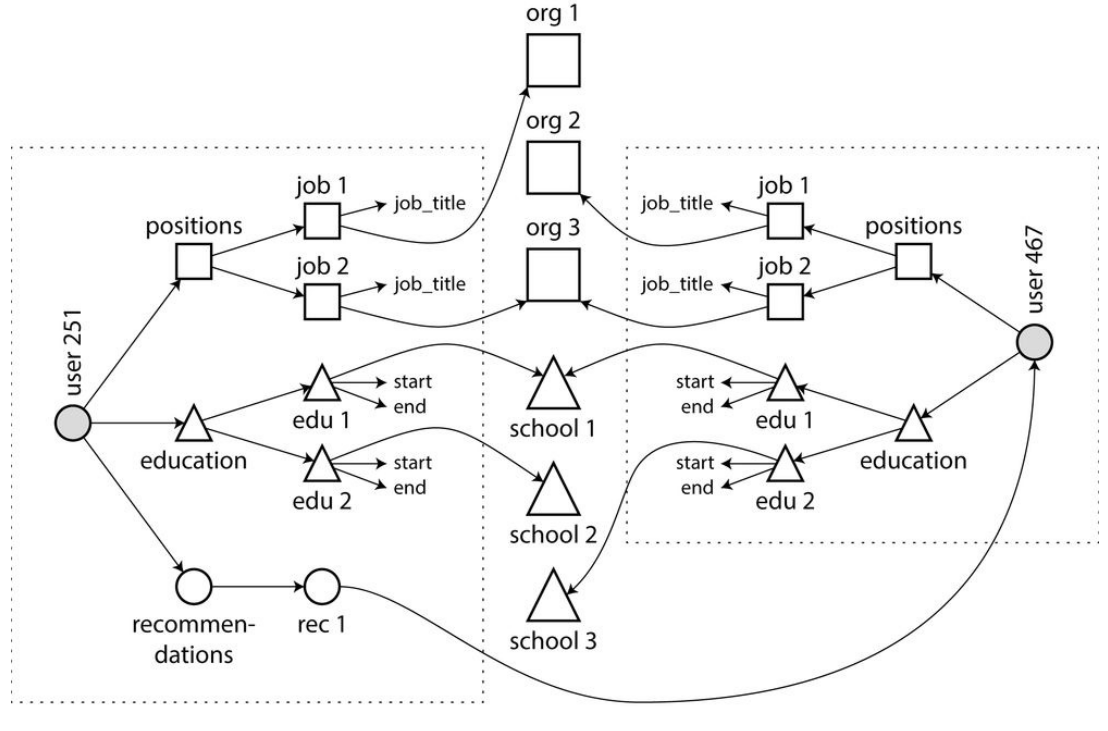
\includegraphics[scale=0.25]{6}
\end{center}

\pagebreak

\subsection{Responder ao aumento do volume de dados}

We are creating, storing, processing more data than ever before!

\vspace{3mm}
Existem duas abordagens possíveis:
\begin{itemize}
  \item Contruir bases de dados mauores;
  \item Criar um grupo de máquinas mais pequenas que se complementam;
\end{itemize}

\begin{enumerate}
  \item A primeira abordagem tem alguns problemas, uma vez que o \textbf{custo}
  de duplicar a capacidade de uma DB é geralmente mais do dobro do custo de uma
  DB "normal" e mesmo com recursos financeiros, há \textbf{limitações físicas} e de
  engenharia à sua capacidade;
  
  \item A segunda, apesar de mais exequível, tem também alguns defeitos, uma vez
  que por ser uma solução \textbf{barata}, pode refletir-se em \textbf{menos
  fiabilidade}. É ainda nexessário a integração com um DBMS compatível com
  a tipologia.
\end{enumerate}

Os Sistemas de Gestão de Bases de Dados (DBMS) têm alguma \textbf{dificuldade em gerir a escalabilidade
horizontal} (distribuição da BD).

\subsection{O movimento NoSQL}

Este movimento, cujo acrónimo significa
\textbf{Not only SQL}, pretende promover a utilização de bases
de dados não relacionais (SQL). Tem por base vários princípios.

\begin{enumerate}
  \item \textbf{Não é relacional} - Podem ser mas não são boas nisso;
  \item \textbf{API simples} - Sem necessidade de realizar \uline{join};
  \item \textbf{Teorema BASE \& CAP} - Viola os princípios ACID;
  \item \textbf{Schema-free} - Esquema implícito e gerido pela aplicação (sem verificações do lado da DB);
  \item \textbf{Distribuídas} - Algumas mais do que outras;
  \item \textbf{Open-source} - Mostly;
\end{enumerate}

\subsubsection{Transações BASE}

Este acrónimo nasceu em oposição aos princípios ACID, principalmente
em resposta às limitações de consistência que um cenário de um sistema
distribuído impõe.

\begin{itemize}
  \item \textbf{\uline{B}asic \uline{A}vailability} - A DB funciona a maior parte do tempo;
  \item \textbf{\uline{S}oft-state} - As manipulações dos dados não têm de ser write-consistent, nem
  diferentes réplicas têm de ser mutualmente consistentes o tempo todo.
  Escritas num nó da base de dados não têm de ser escritas garantidamente em simultâneo nos restantes nós;
  \item \textbf{\uline{E}ventual consistency} - O armazenamento de dados eventualmente torna-se consistente, em algum ponto
  (e.g. lazily at read time);
\end{itemize}

As bases de dados NoSQL caracterizam-se então por ser \textbf{otimistas} e \textbf{simples}, o que torna a
base de dados mais \textbf{rápida}, \textbf{disponibilidade em primeiro lugar}, \textbf{best effort} e \textbf{appoximate answers OK}.

\pagebreak

\subsubsection{Teorema CAP (Brewer's)}

Este teorema diz que um sistema distribuído só pode apresentar duas de três características:

\begin{itemize}
  \item \textbf{\uline{C}onsistent} - Escritas atómicas em toda a DB em simultâneo;
  \item \textbf{\uline{A}vailable} - A DB responde sempre a pedidos;
  \item \textbf{\uline{P}artition Tolerant} - O sistema consegue funcionar mesmo que um nó deixe de responder;
\end{itemize}

\begin{center}
  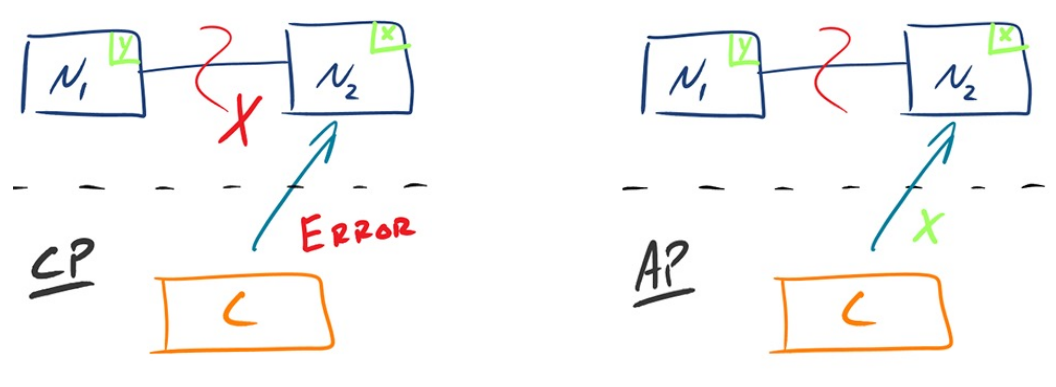
\includegraphics[scale=0.3]{7}
\end{center}

\begin{flushleft}
  \begin{enumerate}
    \item No primeiro temos uma base de dados que implementa a consistência e a tolerância a falhas.
    Quando um cliente faz um pedido de consulta de um valor, caso o nó não consiga contactar os restantes de forma a
    confirmar que todos têm o mesmo valor, retorna uma mensagem de erro.
    \item No segundo temos a disponibilidade e tolerância a falhas. Neste caso, mesmo com uma falha de comunicação entre
    os nós, o nó contactado pelo cliente vai responder com o valor pedido, mesmo que este não seja o mai atual.
  \end{enumerate}
\end{flushleft}

\begin{center}
  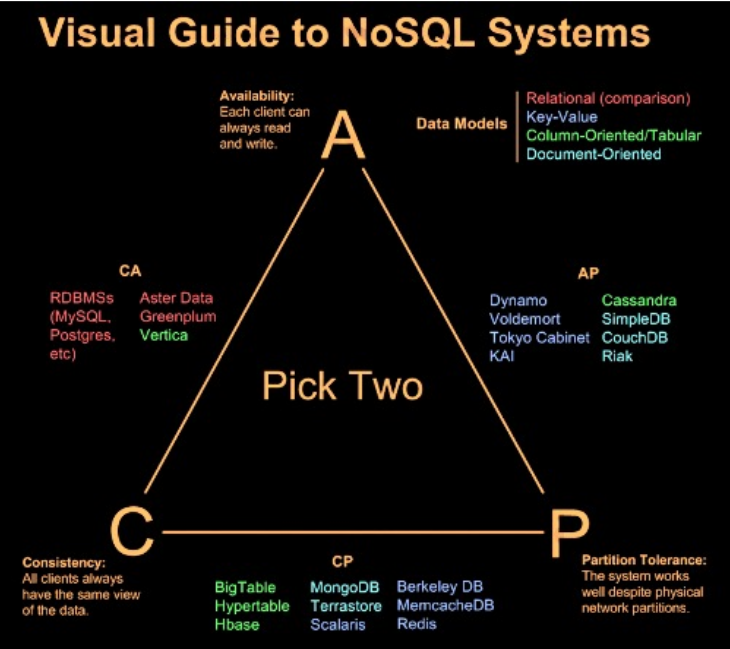
\includegraphics[scale=0.3]{8}
\end{center}

\pagebreak

\subsection{Tipos de Bases de Dados NoSQL}


\end{document}